\chapter{Décroissances nucléaires}
\section{Généralités}
Passons en revue les différents processus de décroissances nucléaires
\begin{description}
\item[Radioactivité $\alpha$] Émission d'une particule $^4$He ($Z=N=2$). Celle-ci est limitée par la 
barrière coulombienne. Exemple = $^238$U ($Z=92$) $\to$ $^{234}$Th ($Z=90$) + $\alpha$.
\item[Radioactivité $\beta$] Émission d'un électron ou d'un position (et d'un neutrino). 
\item[Radioactivité $\gamma$] Résulte de l'interaction électromagnétique
\item[Fission] Analogue à la décroissance $\alpha$ (rare à cause de la barrière coulombienne)
\end{description}\ 

Ces différentes décroissances possèdes deux caractéristiques ((très) variable en fonction du processus) : 
l'énergie de seuil $Q$ (différence d’énergie entre les états initial et final) et la durée de vie.\\

On décroit la décroissance d'un échantillon de $N$ éléments par le \textbf{taux de désintégration par
unité de temps} $\lambda$ ([s$^{-1}$]). Le nombre de désintégration durant un temps $dt$ est donné par
$\lambda$d$t$ et forcément, le nombre d'éléments qui disparaissent d$N : -\lambda Ndt$. Après un calcul
d'une complexité absolue, on en tire
\begin{equation}
N(t) = N_0\exp(-\lambda t)
\end{equation}
où $N_0$ est le nombre initial d'éléments. On défini la \textbf{demi-vie}
\begin{equation}
N(T_{1/2}) = \frac{N_0}{2}) \to T_{1/2} = \frac{\ln 2}{\lambda}
\end{equation}
Le \textbf{temps de vie moyen} s'écrit alors 
\begin{equation}
\tau = \frac{\int t N(t)dt}{\int  N(t)dt} = \frac{1}{\lambda} = \frac{T_{1/2}}{\ln 2} \approx 1.44\times T_{1/2}
\end{equation}

Il existe trois unités conventionnelles : le Curie ($3.7\times 10^{10}$ désintégrations/s), le
Rutherford (($10^{6}$ désintégrations/s) et le Becquerel (1 désintégration/s). Il est possible de 
généraliser ce que nous venons de voir au cas où il existe plusieurs voies de décroissances. En effet, un
même noyau peut avoir plusieurs modes de décroissances avec des probabilités $\lambda_1,\lambda_2,\dots$. La
probabilité totale est donnée par $\lambda_T = \lambda_+\lambda_2+\dots$ et la durée de vie par
$\tau_T = \frac{1}{T}=\frac{1}{\tau_1}+\frac{1}{\tau_2}+\dots$ On utilise parfois les rapports de branchement,
sans dimension : $\lambda_i/\lambda_T$.\\

Les méthodes de datations étudient le passage d'un élément 1 à un élément 2. A l'instant $t_0 : N_1(t_0)$. A 
l'instant $t_1 : N_1(t_1)+N_2(t_1)=N_1(t_0)$ où $N_1(t_1) = N_1(t_0)\exp(-\lambda(t_1-t_0))$. On en déduit
\begin{equation}
\frac{N_1(t_0)}{N_1(t_1)} = 1 +\frac{N_2(t_1)}{N_1(t_1)} = \exp(\lambda(t_1-t_0))
\end{equation}
La mesure de $N_2$ et $N_1$ à l'instant $t_1$ permet de déduire $t_0$. Actuellement on procède à un comptage
précis des quantités par réaction nucléaire. En pratique ceci n'est pas valable pour des longues durées de 
vies ($N_1$ peut continuer à être formé) et on mesurera des rapports de nombres d'éléments.

\section{Notion de largeur}
Considérons une onde stationnaire, représentant un système restant indéfiniment dans le même état
\begin{equation}
\Psi(r,t) = \Psi(r)\exp\left(-\frac{iE_0t}{\hbar}\right) \quad\Rightarrow\quad |\Psi(r,t)|^2 = |\Psi(r)|^2
\end{equation}
où la fonction d'onde est donné par le produit d'une partie spatiale et d'une phase dépendante de l'énergie.\\

S'il y a une décroissance, le nombre de particule va varier avec le temps. Si cette décroissance se fait avec une
constante $\lambda$, la dépendance sera la suivante
\begin{equation}
|\Psi(r,t)|^2 = |\Psi(r,0)|^2\exp(-\lambda t)
\end{equation}
Dès lors, la partie temporelle de notre fonction d'onde est modifiée 
\begin{equation}
\Psi(r,t) = \Psi(r)\exp\left(-\frac{it}{\hbar}\left(E_0-\frac{i\lambda\hbar}{2}\right)\right)
\end{equation}
ce qui forme un état non-stationnaire (état \textbf{résonant}). Cette modification vient du fait que l'énergie
à été modifiée : tout se passe comme si l'énergie était complexe
\begin{equation}
W = E_0-\frac{i\lambda\hbar}{2}
\end{equation}
où la partie imaginaire imaginaire reprend la dépendance $\lambda$ et est donc liée au taux de décroissance. Si
ce taux est très petit (cas réel) seul la partie réelle est à prendre en compte mais si $\lambda$ est très grand, 
la partie imaginaire est à prendre en compte. En mécanique quantique, on utilise des énergies réelles. On 
exprime alors la superposition d'ondes stationnaires à énergie réelles
\begin{equation}
\exp\left(-\frac{it}{\hbar}\left(E_0-\frac{i\lambda\hbar}{2}\right)\right) = \int A(E)\exp\left(
-\frac{itE}{\hbar}\right)\text{ d}E
\end{equation}

	\begin{wrapfigure}[11]{r}{5cm}
	\vspace{-5mm}
	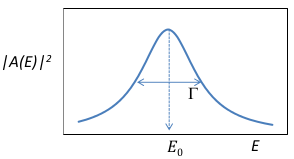
\includegraphics[scale=0.45]{ch4/image1}
	\captionof{figure}{Énergie complexe $W=E_0-i\Gamma/2$. Résonance large : $\Gamma$ grand, $\tau$ petit et 
	inversément pour une étroite}
	\end{wrapfigure}

Ceci permet de déterminer l'amplitude $A(E)$ par transformée de \textsc{Fourier} inverse. On obtient alors
\begin{equation}
|A(E)|^2 = \dfrac{1}{4\pi^2}\dfrac{1}{(E-E_0)^2+\Gamma^2/4}
\end{equation}
Sachant que la largeur à mi-hauteur vaut $\Gamma = \hbar\lambda = \frac{\hbar}{\tau}$, il est possible de 
recombiner les deux pour obtenir une relation d'incertitude ressemblant à celle d'\textsc{Heisenberg} :
$\Gamma \tau = \hbar$. On trouve les états stable pour $\Gamma =0,\tau=\infty, A(E)\propto \delta(E-E_0)$. Les
états instables sont obtenus par superposition d'une infinité d'états stationnaires et ils sont caractérisés
par une énergie $E_0$ et une largeur $\Gamma$.











\newpage
\section{Règle d'or de Fermi}
La règle d'or de \textsc{Fermi} permet de calculer la probabilité de transition entre un état initial $i$ et 
un état final $f$ lorsque l'on perturbe le système par un potentiel petit\footnote{Le principe et très général
et applicable aux transition $\beta$ et $\gamma$. Tous les calculs ne seront pas détaillés ici (assez long et
horrible), mais un "juste milieu" est proposé afin de ne pas juste "plaquer" les formules comme elles viennent}.
Supposons $H=H_0+V$ où $V$ est petit (perturbation) et responsable de la décroissance (stable si $V=0$). On 
suppose également que les états propres de $H_0$ sont connus : $H_0\Psi_n=E_n\Psi_n$. La fonction d'onde est 
solution de 
\begin{equation}
i\hbar\dfrac{\partial\Psi}{\partial t} = H\Psi
\end{equation}
Posons $\DS \Psi(\vec{r},t) = \sum_n a_n(t)\Psi_n(\vec{r})e^{-\frac{iE_nt}{\hbar}}$. En développant ceci
dans la base des états stationnaires, on peut en tirer un système d'équations de \textsc{Schrödinger} donnant
les coefficient $a_k$ (on recherche leurs évolutions dans le temps car ceux-ci donnent les probabilités de
transition)
\begin{equation}
\frac{da_k}{dt} = -\frac{i}{\hbar}\sum_{n}a_n \bra{\Psi_k}V\ket{\Psi_n}e^{\frac{i(E_k-E_n)t}{\hbar}}
\end{equation}
Il s'agit d'un système d'équation linéaires qui dépend des énergies et des éléments de matrice du potentiel
de perturbation. Si on le connaît, on peut en déduire les fonctions d'ondes et en calculer les éléments de
matrice. On va donc procéder par itérations
\begin{equation}
\dfrac{da_k^{(p+1)}}{dt}\approx -\frac{i}{\hbar}\sum_n a_n^ {(p)}
\bra{\Psi_k}V\ket{\Psi_n}e^{\frac{i(E_k-E_n)t}{\hbar}}
\end{equation}
On utilisera comme ordre 0 ($p=0$, condition initiale) $a_n^{(0)} = \delta_{ni}$.\\

	\begin{wrapfigure}[11]{r}{5cm}
	\vspace{-7mm}
	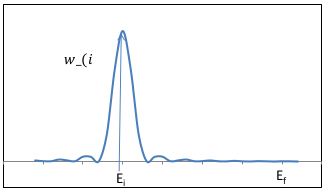
\includegraphics[scale=0.45]{ch4/image2}
	\captionof{figure}{On remarque de légères fluctuations}
	\end{wrapfigure}

Le calcul détaillé donne
\begin{equation}
w_{i\to f} = \dfrac{|a_f|^2}{T}=\frac{1}{T}\dfrac{|V_{fi}|^2}{(E_f-E_i)^2}4\sin^2\frac{(E_f-E_i)T}{2\hbar}
\end{equation}
Lorsque $T$ est grand, $E_f=E_i$ et on retrouve bien la conservation de l'énergie. Notons que $E_i$ et $E_f$ 
sont les énergies du système total. Dans une transition $\gamma, E_i$ est l'état nucléaire initial alors
que $E_f$ est l'état nucléaire final \textbf{et} le photon.\\

Certains noyaux ont une très grande densité d'états et d'autres une très petite. La probabilité de transition
totale s'obtient en sommant sur tous les états finaux possible. Comme dans un cas général on peut avoir
quelque chose de continu, on utilisera le formalisme intégral ($dn=\rho(E_k)dE_k$)
\begin{equation}
w_{i\to f} = \int|w_{i\to k}|^2 \rho(E_k)dE_k
\end{equation}
où l'état $k$ est proche de l'état $f$, $\rho(E_k)$ est la densité d'état à $E_k$ et 
$\rho(E_k)dE_k$ est le nombre d'états dans l'intervalle d$E_k$. On en déduit\footnote{Voir cours 
\textsc{Mécanique quantique I} pour un calcul plus détaillé}
\begin{equation}
w_{i\to f} = \dfrac{4}{T}\int\dfrac{\sin^2\frac{(E_k-E_i)T}{2\hbar}}{(E_k-E_i)^2}|V_{ki}|^2\rho(E_k)dE_k
\end{equation}
Il s'agit du carré de la fonction \textit{sinus cardinal} qui est dominante pour $x=0$ et définie telle 
que $\int_{-\infty}^\infty \text{sinc}^2(x)\text{d}x=\pi$. Sachant ceci et en supposant que 
$V_{ki}\approx V_{fi}$ et que $\rho(E_k)$ varie peu autour de $E_i$, on peut en trouver un résultat final
qui est la règle d'or de \textsc{Fermi}\\

\cadre{\textsc{Règle d'Or de Fermi} (formule générale)
\begin{equation}
w_{i\to f} = \lambda = \frac{2\pi}{\hbar}|\bra{\Psi_i}V\ket{\Psi_f}|^2\rho(E_i)
\end{equation}}


Terminons par un petit commentaire sur les ordres de grandeur et la "hiérarchie" : comme la probabilité de
transition est liée a des éléments de matrice impliquant le potentiel, on s'attend à ce qu'elle respecte un 
certain "ordre". Les largeurs $\alpha$ sont en générales plus grande que les $\gamma$ qui elles sont plus 
grandes que mes $\beta$. Cette hiérarchie est respectée dans les types de potentiels.\\

A partir de $\lambda$, on en déduit la durée de vie $T=1/\lambda$ et la largeur $\Gamma = \hbar/T=\hbar\lambda$.
\begin{itemize}
\item[$\bullet$] Radioactivité $\alpha$ : $V=V_{nuc}$ ($V\ll H_0$, règle d'or \textbf{pas} valable pour $\alpha$)
\item[$\bullet$] Radioactivité $\beta$ : $V=V_{faible}$ 
\item[$\bullet$] Radioactivité $\gamma$ : $V=V_{elec}$ 
\end{itemize}\

En général, comme dit ci-dessus
\begin{equation}
\Gamma_\alpha > \Gamma_\gamma > \Gamma_\beta
\end{equation}

\begin{center}
	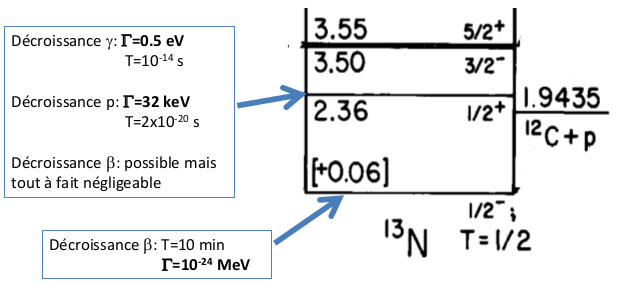
\includegraphics[scale=0.45]{ch4/image3}
	\captionof{figure}{Spectre du $^{13}$N (13 protons et 6 neutrons). Le premier état excité a une énergie de 
	2.36 MeV. L'état fondamental à une masse plus petite que $^{12}$C + $p$, il s'agit donc d'une voie de
	désintégration possible.}
\end{center}







